\documentclass[12pt,a4paper]{report}

\usepackage[utf8]{inputenc} % pentru suport diacritice
\usepackage[romanian]{babel} % setări pentru limba română 
\renewcommand\familydefault{\sfdefault} % sans serif

\usepackage[margin=2.54cm]{geometry}	% dimensiuni pagină și margini
\usepackage{graphicx} % support the \includegraphics command and options

% formatting sections and subsections
\usepackage{textcase}
\usepackage{hyphenat}
\usepackage[titletoc, title]{appendix}
\usepackage{titlesec}
\titleformat{\chapter}{\large\bfseries\MakeUppercase}{\thechapter}{2ex}{}[\vspace*{-1.5cm}]
\titleformat*{\section}{\large\bfseries}
\titleformat*{\subsection}{\large\bfseries}
\titleformat*{\subsubsection}{\large\bfseries}

\usepackage{chngcntr}
\counterwithout{figure}{chapter} % no chapter number in figure labels
\counterwithout{table}{chapter} % no chapter number in table labels
\counterwithout{equation}{chapter} % no chapter number in equation labels

\usepackage{booktabs} % for much better looking tables
\usepackage{url} % Useful for inserting web links nicely
\usepackage[bookmarks,unicode,hidelinks]{hyperref}

\usepackage{array} % for better arrays (eg matrices) in maths
\usepackage{paralist} % very flexible & customisable lists (eg. enumerate/itemize, etc.)
\usepackage{verbatim} % adds environment for commenting out blocks of text & for better verbatim
\usepackage{subfig} % make it possible to include more than one captioned figure/table in a single float
\usepackage{enumitem}
\setlist{noitemsep}

%%% HEADERS & FOOTERS
\usepackage{fancyhdr}
\pagestyle{empty}
\renewcommand{\headrulewidth}{0pt}
\renewcommand{\footrulewidth}{0pt}
\lhead{}\chead{}\rhead{}
\lfoot{}\cfoot{\thepage}\rfoot{}



\newcommand{\HeaderLineSpace}{-0.25cm}
\newcommand{\UniTextRO}{UNIVERSITATEA POLITEHNICA DIN BUCUREȘTI \\[\HeaderLineSpace] 
FACULTATEA DE AUTOMATICĂ ȘI CALCULATOARE \\[\HeaderLineSpace]
DEPARTAMENTUL DE CALCULATOARE\\}
\newcommand{\DiplomaRO}{PROIECT DE DIPLOMĂ}
\newcommand{\AdvisorRO}{Coordonator științific:}
\newcommand{\BucRO}{BUCUREȘTI}

\newcommand{\UniTextEN}{UNIVERSITY POLITEHNICA OF BUCHAREST \\[\HeaderLineSpace]
FACULTY OF AUTOMATIC CONTROL AND COMPUTERS \\[\HeaderLineSpace]
COMPUTER SCIENCE AND ENGINEERING DEPARTMENT\\}
\newcommand{\DiplomaEN}{DIPLOMA PROJECT}
\newcommand{\AdvisorEN}{Thesis advisor:}
\newcommand{\BucEN}{BUCHAREST}

\newcommand{\frontPage}[6]{
\begin{titlepage}
\begin{center}
{\Large #1}  % header (university, faculty, department)
\vspace{50pt}
\begin{tabular}{p{6cm}p{4cm}}

\includegraphics[scale=0.8]{pics/upb-logo.jpg} &
	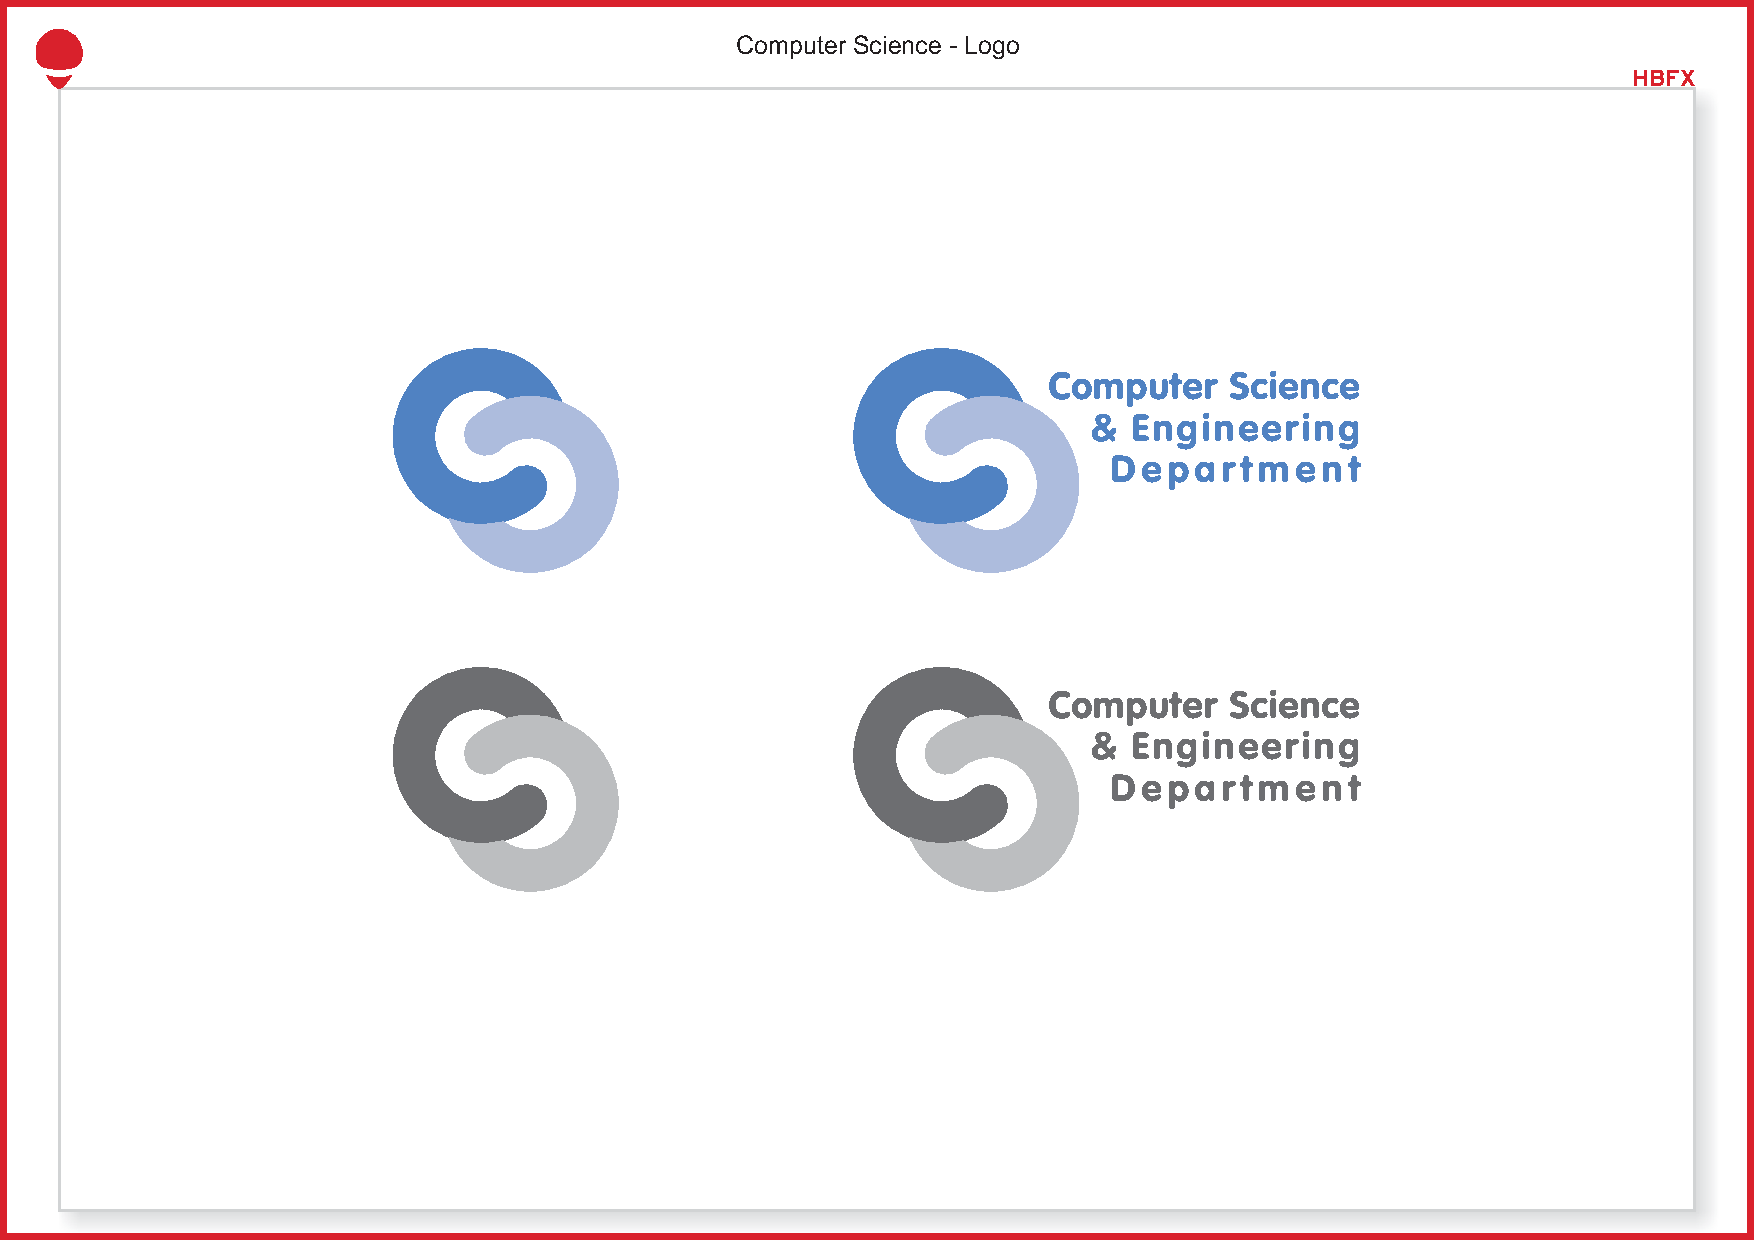
\includegraphics[scale=0.5,trim={14cm 11cm 2cm 5cm},clip=true]{pics/cs-logo.pdf}
\end{tabular}

\vspace{105pt}
{\Huge #2}\\                           % diploma project text
\vspace{40pt}
{\Large #3}\\ \vspace{0pt}  % project title
{\Large #4}\\                          % project subtitle
\vspace{40pt}
{\LARGE \Name}\\                   % student name
\end{center}
\vspace{60pt}
\begin{tabular*}{\textwidth}{@{\extracolsep{\fill}}p{6cm}r}
&{\large\textbf{#5}}\vspace{10pt}\\      % scientific advisor
&{\large \Advisor}                                    % advisor name
\end{tabular*}
\vspace{20pt}
\begin{center}
{\large\textbf{#6}}\\                                % bucharest
\vspace{0pt}
{\normalsize \Year}
\end{center}
\end{titlepage}
}

\newcommand{\frontPageRO}{\frontPage{\UniTextRO}{\DiplomaRO}{\ProjectTitleRO}{\ProjectSubtitleRO}{\AdvisorRO}{\BucRO}}
\newcommand{\frontPageEN}{\frontPage{\UniTextEN}{\DiplomaEN}{\ProjectTitleEN}{\ProjectSubtitleEN}{\AdvisorEN}{\BucEN}}

\linespread{1.15}
\setlength\parindent{0pt}
\setlength\parskip{.28cm}

%% Abstract macro
\newcommand{\AbstractPage}{
\begin{titlepage}
\textbf{\large SINOPSIS}\par
\AbstractRO\par\vfill
\textbf{\large ABSTRACT}\par
\AbstractEN \vfill
\end{titlepage}
}

%% Thank you macro
\newcommand{\ThanksPage}{
\begin{titlepage}
{\noindent \large\textbf{MULȚUMIRI}}\\
\Thanks
\end{titlepage}
}



%%%%%%%%%%%%%%%%%%%%%%%%%%%%%%%%%%%%%%%%%%%%%%%%%%   
%%
%%          End of template definitions
%%   
%%%%%%%%%%%%%%%%%%%%%%%%%%%%%%%%%%%%%%%%%%%%%%%%%%


%%% Puteți elimina aceste linii din lucrare, servesc numai pentru template.
\newcommand{\worktype}[1]{[\textit{#1}] }
\newcommand{\dezvoltare}{\worktype{Dezvoltare de produs}}
\newcommand{\cercetare}{\worktype{Cercetare}}
\newcommand{\ambele}{\worktype{Ambele}}
%%%


%%
%%   Campurile de mai jos trebuie modificate de autor. Modificati doar continutul, nu si numele fiecarei definitii
%%
\newcommand{\ProjectTitleRO}{Titlul proiectului de diplomă (ex: Șablon proiect de diplomă)}
\newcommand{\ProjectSubtitleRO}{Subtitlu (ex: versiunea 2018)}
\newcommand{\ProjectTitleEN}{Diploma Project Title  (eg: Diploma project template)}
\newcommand{\ProjectSubtitleEN}{Subtitle (eg: 2018 version)}
\newcommand{\Name}{Ioana Popescu}
\newcommand{\Advisor}{Prof. dr. ing. Andrei Ionescu}
\newcommand{\Year}{2018}

% Setări document
\title{Proiect de diplomă}
\author{\Name}
\date{\Year}

%%
%%   Campurile aferente rezumatului
%%
\newcommand{\AbstractRO}{Sinopsisul proiectului are rol de introducere, conținând atât o descriere pe scurt a problemei abordate cât și o enumerare sumară a rezultatelor și a concluziilor. Se recomandă ca sinopsisul să fie redactat într-un limbaj accesibil unei persoane nefamiliarizate cu domeniul, dar în același timp destul de specific pentru a oferi rapid o vedere de ansamblu asupra proiectului prezentat.
Sinopsisul proiectului va fi redactat atât în română cât și în engleză. Ca dimensiunea recomandată aceasta secțiune va avea maxim 200 de cuvinte pentru fiecare variantă. Împreună, ambele variante se vor încadra într-o singură pagină.}

\newcommand{\AbstractEN}{The abstract has an introductory role and should engulf both a brief description of the issue at hand, as well as an overview of the obtained results and conclusions. The abstract should be formulated such that even somebody that is unfamiliar with the projects’ domain can grasp the objectives of the thesis while, at the same time, retaining a specificity level offering a bird’s eye view of the project.
The projects’ abstract will be elaborated in both Romanian and English. The recommended size for this section is limited to 200 words for each version. Together, both versions will fit in one page.}

%%
%%   Campurile aferente paginii de multumiri
%%
\newcommand{\Thanks}{(opțional) Aici puteți introduce o secțiunea specială de mulțumiri / acknowledgments. }

\begin{document}

\frontPageRO
\frontPageEN

\begingroup
\linespread{1}
\tableofcontents
\endgroup

\AbstractPage

% poate fi comentata sau stearsa
\ThanksPage


% Textul licentei incepe de aici 



\chapter{Introducere}\pagestyle{fancy}
% * <marios.choudary@gmail.com> 2018-02-28T11:38:18.106Z:
% 
% > INTRODUCERE
% Am scos de aici referintele la font pentru a nu mai fi dependenti de Calibri. Personal, nici nu sunt sigur ca ajuta prea mult aceasta recomandare si mi se pare bun font-ul default din Latex (Computer Modern). Daca sunteti de-acord, va rog sa stergeti liniile comentate de mai jos, precum si cele referitoare la fontul Calibri din restul documentului.
% 
% ^.
Parametrii de formatare recomandați pentru lucrare: 
\begin{itemize}
 %\item Font recomandat: Calibri; Dimensiune font: 12; 
 \item Dimensiune font: 12; 
 \item Spațiere între linii: 1,5; Spațiere după paragraf: 8pt;
 \item Stil: Justified;
 \item Dimensiune pagină: A4; Margini: 2,54cm/ 2,54cm/ 2,54cm/ 2,54cm;
 %\item Heading1: Calibri, 14, bold, all caps;
 %\item Heading2: Calibri, 14, bold;
 %\item Heading3: Calibri, 12. 
 %\item Font pentru formule: Cambria Math, 12.
 \item Heading1: 14, bold, all caps;
 \item Heading2: 14, bold;
 \item Heading3: 12. 
 \item Font size pentru formule: 12.
\end{itemize}
În cadrul introducerii, este necesară abordarea următoarelor puncte care reprezintă de fapt familiarizarea cititorului (comisia, alți colegi sau experți în domeniu) cu tema proiectului, soluția propusa și cuprinsul/structura lucrării. Deși introducerea poate conține și unele elemente mai generale, se recomandă păstrarea unui limbaj tehnic, specific audienței care va citi lucrarea.

În cadrul capitolelor următoare, veți regăsi o serie notații de forma \dezvoltare, \cercetare. Acest tip de formatare este utilizat exclusiv în acest template pentru a marca sfaturi și cerințe specifice pentru lucrări de diploma cu specific diferit. În pregătirea documentului vostru, nu veți utiliza aceste marcaje. 
Elementele pe care trebuie să le abordați în introducere sunt descrise în cadrul subcapitolelor de mai jos. 
\section{Context}
O scurtă introducere a proiectului, motivație, explicație de ce este relevant domeniul proiectului.
\section{Problema} 
Care este problema pe care proiectul o va rezolva.
\section{Obiective}
Care sunt obiectivele proiectului/soluției/abordării/ideii; Ce creșteri sau evoluții determină rezolvarea proiectului.
\section{Soluția propusă} 
Descrierea pe scurt a soluției implementate; ce abordare este propusă (nu detalierea utilitarelor și a tehnologiilor, ci abordarea și ideea propusă de către autor).
\section{Rezultatele obținute}
Descriere pe scurt a rezultatelor obținute, eventual de ce acestea sunt importante față de alte soluții sau studii.
\section{Structura lucrării}
Un paragraf în care fiecare dintre secțiunile următoare este prezentată în 1-2 fraze, punând accentul pe elementele cele mai semnificative din fiecare secțiune.



\chapter{Analiza Cerințelor / Motivație}
\dezvoltare Acest capitol va analiza cerințele produsului din prisma potențialilor clienți și a scenariilor de utilizare preconizate, urmând a fi generată o lista de funcționalități. 

\cercetare Acest capitol va introduce motivația realizării proiectului propus.

Dacă proiectul de licență face parte dintr-un proiect mai amplu (de exemplu un proiect complex, la care lucrează 2 studenți (ex: 1 student la front-end-ul aplicației, 1 student la back-end-ul aplicației), în acest capitol va fi explicat pe scurt ansamblul proiectului și ce parte din proiect este adresată de lucrarea propusă. 

Criterii pentru calificativul \textit{Ne\textit{Satisfăcător}}: 
\begin{itemize}
	\item \dezvoltare Cerințele sunt imaginate de student pe baza unei analize a pieței;
	\item \cercetare Nu se oferă o motivație valida.
\end{itemize}

Criterii pentru calificativul \textit{Satisfăcător}: 
\begin{itemize}
	\item \dezvoltare Există un interviu, un client, analiza cerințelor este elaborată pe baza interviului;
	\item \cercetare Motivația este doar personala.
\end{itemize}


Criterii pentru calificativul \textit{Bine}: 
\begin{itemize}
	\item	 \dezvoltare Proces iterativ pe baza unor interviuri cu mai mulți clienți, dezvoltare MVP, reevaluare cerințe;
	\item	 \cercetare Motivația este legata de o necesitate științifica / tehnica explicită.
\end{itemize}


\chapter{Studiu de Piață / Metode Existente}
\dezvoltare Ce soluții similare există pe piață? Care sunt limitările lor / pentru ce cazuri de utilizare sau pentru ce tip de clienți produsele existente pe piață nu răspund cerințelor? Care sunt indicatorii pe baza cărora sunt evaluate aceste produse, de către potențiali clienți, și unde sunt lipsurile/ care este oportunitatea generată de lipsurile acestea?

\cercetare Metode existente (sau ``State of the Art'') se referă, de regulă, la nivelul curent de dezvoltare: care este starea curentă a domeniului, unde ne găsim, care este contextul. Care sunt soluțiile actuale prezente în literatura de specialitate și care sunt limitările lor? Ce direcții de explorare sunt recomandate în literatura de specialitate? Literatura de specialitate se refera la articole științifice recente, publicate în reviste cu factor de impact mare, sau în volumele unor conferințe de top, sau în cărți.

\ambele În încheierea acestui capitol se dorește descrierea tehnologiilor folosite în lucrare, cu alternative și cu argumente convingătoare calitative și cantitative.  

Criterii pentru calificativul \textit{Ne\textit{Satisfăcător}}: 
\begin{itemize}
	\item \dezvoltare Sunt analizate superficial câteva produse de pe piață; 
	\item \cercetare analiza literaturii limitata la grupuri de cercetare din România;
	\item \ambele Sunt descrise tehnologiile folosite în lucrare. 
\end{itemize}

Criterii pentru calificativul \textit{Satisfăcător}:
\begin{itemize}
	\item \dezvoltare Există un interviu, un client, analiza cerințelor este elaborată pe baza interviului.
	\item \cercetare analiza literaturii de specialitate din lume, fără poziționarea precisă a lucrării în peisajului domeniului studiat;
	\item \ambele Sunt descrise câteva tehnologii alternative pentru fiecare din tehnologiile folosite în lucrare. Există o argumentare referitoare la alegere.
\end{itemize}

Criterii pentru calificativul \textit{Bine}:
\begin{itemize}
	\item \dezvoltare Proces iterativ pe baza unor interviuri cu mai mulți clienți, dezvoltare MVP, reevaluare cerințe;
	\item \cercetare analiza literaturii de specialitate din lume, cu poziționarea precisă a lucrării în peisajul actual al domeniului studiat; 
	\item \ambele Sunt descrise tehnologii alternative. Sunt analizate cantitativ și calitativ, folosite benchmarkuri și teste efectuate de student. Analiza este rezumată prin tabele și grafice.
\end{itemize}

\section{Indicații formatare figuri}

Figurile utilizate în document vor fi centrate și numerotate (de exemplu Figura~\ref{fig:pic1}). 
Orice figură ce nu este realizată de către autorul lucrării va fi în mod obligatoriu citată fie la final (de exemplu Figura ~\ref{fig:pic2} este preluată din documentul \cite{}), fie cel puțin într-o notă de subsol (a se vedea Figura~\ref{fig:pic2}). Orice figură ce depășește ca dimensiune 50\% dintr-o pagină, va fi mutată la anexe. Toate figurile din cadrul tezei vor fi referite în text. Exemplu: Figura~\ref{fig:pic1} prezintă o schemă de principiu pentru un amplificator inversor cu AO. 

\begin{figure}[th]
\centering
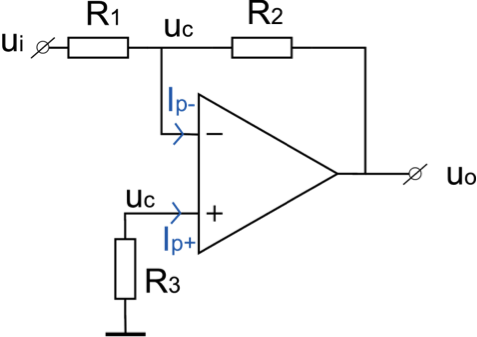
\includegraphics{pics/Pic1.png}
  \caption{Amplificator inversor}
  \label{fig:pic1}
\end{figure}

\newpage

\begin{figure}[th]
\centering
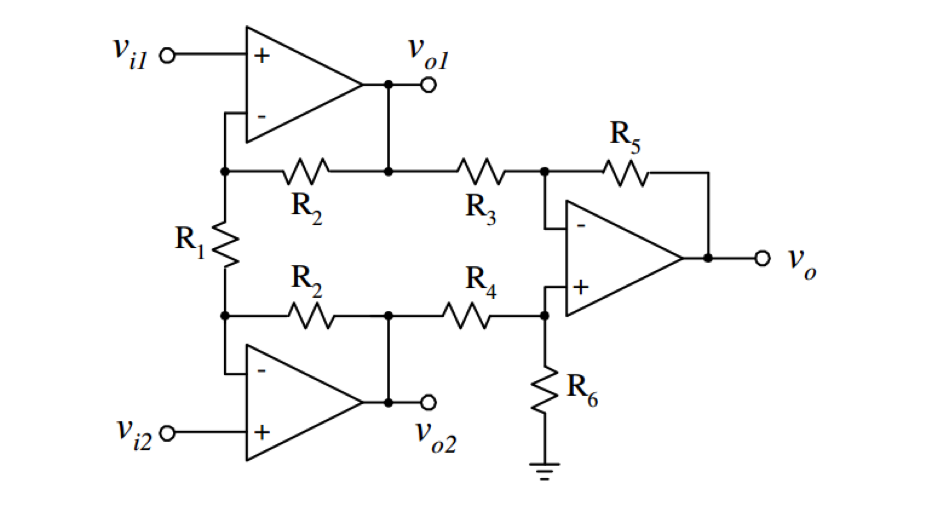
\includegraphics{pics/Pic2.png}
  \caption[Amplificator de instrumentație cu 3 AO-uri]{Amplificator de instrumentație cu 3 AO-uri\protect\footnotemark}
  \label{fig:pic2}
\end{figure}
\footnotetext{© http://www.ece.tamu.edu/sspalermo/ecen3205/Secton\%201III.pdf}

\chapter{Soluția Propusă}
Capitolul conține o privire de ansamblu a soluției ce rezolvă problema, prin prezentarea structurii / arhitecturii acesteia. În funcție de tipul lucrării acest capitol poate conține diagrame (clase, distribuție, workflow, entitate-relație), demonstrații de corectitudine pentru algoritmii propuși de autor, abordări teoretice (modelare matematică), structura hardware, arhitectura aplicației.


Criterii pentru calificativul \textit{Ne\textit{Satisfăcător}}: 
\begin{itemize}
	\item	Descriere în limbaj natural.
\end{itemize}

Criterii pentru calificativul \textit{Satisfăcător}: 
\begin{itemize}
	\item	Descriere + diagrame de baze de date, workflow, clase, algoritmi. 
\end{itemize}

Criterii pentru calificativul \textit{Bine}: 
\begin{itemize}
	\item 	Descriere + diagrame de baze de date, workflow, clase, algoritmi + descrierea unui proces prin care s-a realizat arhitectura/structura soluției.
\end{itemize}

\section{Indicații formatare formule}
Formulele matematice utilizate în document vor fi centrate în pagină și numerotate. 

\begin{equation}
(x+a)^n = \sum_{k=0}^{n}\left(\begin{array}{c}n\\k\\\end{array}\right)x^ka^{n-k}
\end{equation}

\begin{equation}
f(x) = a_0 + \sum_{n=1}^{\infty}\left(a_n \cos\frac{n\pi x}{L} + b_n\sin\frac{n\pi x}{L}\right)
\end{equation}



\chapter{Detalii de implementare}
În plus fata de capitolul precedent acesta conține elemente specifice ale rezolvării problemei care au presupus dificultăți deosebite din punct de vedere tehnic. Pot fi incluse configurații, secvențe de cod, pseudo-cod, implementări ale unor algoritmi, analize ale unor date, scripturi de testare. De asemenea, poate fi detaliat modul în care au fost utilizate tehnologiile introduse in capitolul 3.


Criterii pentru calificativul \textit{Ne\textit{Satisfăcător}}: 
\begin{itemize}
	\item	Sunt prezentate pe scurt scheme și pseudo-cod.
\end{itemize}
Criterii pentru calificativul \textit{Satisfăcător}: 
\begin{itemize}
	\item	Descriere sumara a implementării, prezentarea unor secvențe nerelevante de cod, sch\hyp{}eme, etc. 
\end{itemize}
Criterii pentru calificativul \textit{Bine}: 
\begin{itemize}
	\item	Descrierea detaliată a algoritmilor/structurilor utilizați; Prezentarea etapizată a dezvol\hyp{}tării, inclusiv cu dificultăți de implementare întâmpinate, soluții descoperite; (dacă este cazul) demonstrarea corectitudinii algoritmilor utilizați. 
\end{itemize}

\section{Indicații formatare tabele}
Se recomandă utilizarea tabelelor de forma celui de mai jos.  Font size :  9. 
Orice tabel prezent în teză va fi referit în text; exemplu: a se vedea Tabel~\ref{tab:criterii}.

\begin{table}[th]\small\linespread{1}
\caption{Sumarizare criterii}
\label{tab:criterii}
\begin{tabular}{l >{\raggedright\arraybackslash}p{8cm} >{\raggedright\arraybackslash}p{4cm}}
\textbf{Calificativ} & \textbf{Criteriu} & \textbf{Observații} \\\hline
\textbf{Nesatisfacator} & Sunt prezentate pe scurt scheme și pseudo-cod & \\\hline
\textbf{Satisfacator} &Descriere sumara a implementării, prezentarea unor secvențe nerelevante de cod, scheme, etc.& \\
\hline
\textbf{Bine} &Descrierea detaliată a algoritmilor/structurilor utilizați; Prezentarea etapizată a dezvoltării, inclusiv cu dificultăți de implementare întâmpinate, soluții descoperite; (dacă este cazul) demonstrarea corectitudinii algoritmilor utilizați. & Pot fi incluse configurații, secvente de cod, pseudo-cod, implementări ale unor algoritmi, analize ale unor date, scripturi de testare. \\
\hline
\end{tabular}
\end{table}


\chapter{Evaluare}
Acest capitol trebuie să răspundă, în principiu, la 2 întrebări și să se încheie cu o discuție a rezultatelor obținute. Cele doua întrebări la care trebuie sa se răspundă sunt:
\begin{enumerate}
	\item  \textbf{Merge corect?} (Conform specificațiilor extrase în capitolul 2); 
Evaluarea dacă merge corect se face pe baza cerințelor identificate în capitolele anterioare. 

	\item Cât de \textit{Bine} merge / cum se compară cu soluțiile existente? (pe baza unor metrici clare). 
Evaluarea cât de \textit{Bine} merge trebuie să fie bazată pe procente, timpi, cantitate, numere, \textbf{comparativ cu soluțiile prezentate în capitolul 3}. Poate fi vorba de performanță, overhead, resurse consumate, scalabilitate etc. 
\end{enumerate}

În realizarea discuției, se vor utiliza tabele cu procente, rezultate numerice și grafice. În mod obișnuit, aici se fac comparații și teste comparative cu alte proiecte similare (dacă există) și se extrag puncte tari și puncte slabe. Se ține cont de avantajele menționate și se demonstrează viabilitatea abordării / aplicației, de dorit prin comparație cu alte abordări (dacă acest lucru este posibil). Cuvântul cheie la evaluare este ``metrică'': trebuie să aveți noțiuni măsurabile și cuantificabile. În cadrul procesului de evaluare, explicați datele, tabelele și graficele pe care le prezentați și insistați pe relevanța lor, în următorul stil: ``este de preferat ... deoarece …''; explicați cititorului nu doar datele ci și semnificația lor și cum sunt acestea interpretate. Din această interpretare trebuie să rezulte poziționarea proiectului vostru printre alternativele existente, precum și cum poate fi acesta îmbunătățit în continuare.

Criterii pentru calificativul \textit{Ne\textit{Satisfăcător}}: 
\begin{itemize}
	\item Aplicația este testată dar rulează pe calculatorul studentului, nu există posibilități de testare, nu a fost validată cu clienți / utilizatori;
	\item Nu au fost realizate comparații cu alte sisteme similare.
\end{itemize}

Criterii pentru calificativul \textit{Satisfăcător}: 
\begin{itemize}
	\item \dezvoltare  Există teste unitare și de integrare, există o strategie de punere în funcțiune (deployment), există validare minimală cu clienții / utilizatorii.
	\item \cercetare Principalele componente și soluția în ansamblu au fost evaluate din punct de vedere al performanței, însă nu sunt folosite seturi de date standard, există unele erori de interpretare a datelor.
	\item \ambele Discuție minimală asupra relevanței rezultatelor prezentate, comparație minimală cu alte sisteme similare.
\end{itemize}

Criterii pentru calificativul \textit{Bine}: 
\begin{itemize}
	\item \dezvoltare Teste unitare și de integrare, instrumente de punere in funcțiune (deployment) utilizate și care arată lucru constant de-a lungul semestrului, lucrare validată cu clienții / utilizatorii, produs în producție.
	\item \cercetare Componentele și soluția în ansamblu au fost evaluate din punct de vedere al performanței, folosind seturi de date standard și cu o interpretare corectă a rezultatelor.
	\item \ambele Discuție cu prezentarea calitativă și cantitativă a rezultatelor, precum și a relevanței acestor rezultate printr-o comparație complexă cu alte sisteme similare.
\end{itemize}

\chapter{Concluzii}
În acest capitol este sumarizat întreg proiectul, de la obiective, la implementare, si la relevanta rezultatelor obținute. În finalul capitolului poate exista o subsecțiune de ``Dezvoltări ulterioare''.

Criterii pentru calificativul \textit{Ne\textit{Satisfăcător}}: 
\begin{itemize}
	\item	Concluziile nu sunt corelate cu conținutul lucrării;
\end{itemize}

Criterii pentru calificativul \textit{Satisfăcător}: 
\begin{itemize}
	\item	Concluziile sunt corelate cu conținutul lucrării, însă nu se oferă o imagine asupra calității și relevantei rezultatelor obținute;
\end{itemize}

Criterii pentru calificativul \textit{Bine}: 
\begin{itemize}
	\item	Concluziile sunt corelate cu conținutul lucrării, și se oferă o imagine precisa asupra relevantei și calității rezultatelor obținute în cadrul proiectului. 
\end{itemize}

\chapter*{Bibliografie}\addcontentsline{toc}{chapter}{Bibliografie}  
% * <marios.choudary@gmail.com> 2018-02-28T12:07:48.730Z:
% 
% > BIBLIOGRAFIE
% Am adaugat un paragraf cu cateva detalii despre folosirea citarilor bibliografice in Latex, despre folosirea lui "\cite" si despre posibilitatea folosirii bibliografiei si direct in fisierul Latex.
% 
% ^.

\begin{itemize}
	\item 	NU utilizați referințe la Wikipedia sau alte surse fără autor asumat.
	\item 	Pentru referințe la articole relevante accesibile în web (descrise prin URL) se va nota la bibliografie și data accesării.
	\item 	Mai multe detalii despre citarea referințelor din internet se pot regăsi la:
	\begin{itemize}
		\item	\url{http://www.writinghelp-central.com/apa-citation-internet.html}
		\item	\url{http://www.webliminal.com/search/search-web13.html}
	\end{itemize}
	\item 	Note de subsol se utilizează dacă referiți un link mai puțin semnificativ o singură dată; Dacă nota este citată de mai multe ori, atunci utilizați o referință bibliografică.
	\item 	Dacă o imagine este introdusă în text și nu este realizată de către autorul lucrării, trebuie citată sursa ei (ca notă de subsol sau referință - este de preferat utilizarea unei note de subsol).
	\item 	Referințele se pun direct legate de text (de exemplu ``KVM [1] uses'', ``as stated by Popescu and Ionescu [12]'', etc.). Nu este recomandat să folosiți formulări de tipul ``[1] uses'', ``as stated in [12]'', ``as described in [11]'' etc..
	\item 	Afirmațiile de forma ``are numerous'', ``have grown exponentially'', ``are among the most used'', ``are an important topic'' trebuie să fie acoperite cu citări, date concrete si analize comparative.
	\begin{itemize}
		\item	Mai ales în capitolele de introducere, ``state of the art'', ``related work'' sau ``background'' trebuie să vă argumentați afirmațiile prin citări. Fiți autocritici și gândiți-vă dacă afirmațiile au nevoie de citări, chiar și cele pe care le considerați evidente.
		\item	Cea mai mare parte dintre citări vor fi în capitolele de introducere ``state of the art'', ``related work'' sau ``background''.
	\end{itemize}
	\item 	Toate intrările bibliografice trebuie citate în text. Nu le adăugați pur și simplu la final.
	\item 	Nu copiați sau traduceți niciodată din surse de informație de orice tip (online, offline, cărți, etc.). Dacă totuși doriți să oferiți, prin excepție, un citat celebru - de maxim 1 frază- utilizați ghilimele și evident menționați sursa. .
	\item 	Dacă reformulați idei sau creați un paragraf rezumat al unor idei folosind cuvintele voastre, precizați cu citare (referință bibliografică) sau cu notă de subsol sursa sau sursele de unde ați preluat ideile.
\end{itemize}

Trebuie respectat un singur standard de trimiteri bibliografice (citare), dintre următoarele alternative:
\begin{itemize}
	\item APA (\url{http://pitt.libguides.com/c.php?g=12108\&p=64730})
	\item IEEE (\url{https://ieee-dataport.org/sites/default/files/analysis/27/IEEE\%20Citation\%20Guidelines.pdf}) 
	\item Harvard (\url{https://libweb.anglia.ac.uk/referencing/harvard.htm})
	\item Cu numerotarea referințelor în ordine alfabetică sau în ordinea apariției în text (de exemplu, stilul cu numere folosit de unele publicații ACM - \url{https://www.acm.org/publications/authors/reference-formatting}) 
\end{itemize}

În Latex este foarte ușor să folosiți referințe într-un mod corect și unitar, fie prin adăugarea unei secțiuni
\verb!\begin{thebibliography}!
(vezi la sfârșitul acestei secțiuni), fie printr-un fișier separat de tip bib, folosind comanda
\verb!\bibliography{}!,
așa cum procedăm mai jos prin folosirea fișierului ``bibliography.bib''. În orice caz, în Latex va trebui să folosiți comanda
\verb!\cite{}!
pentru a adăuga referințe, iar această comandă trebuie folosită direct în text, acolo unde vreți sa apară citația, ca în exemplele următoare:
\begin{itemize}
	\item Articol jurnal: ~\cite{article};
	\item Articol conferință:~\cite{proc};
	\item Carte: ~\cite{book};
	\item Weblink: ~\cite{silva};
\end{itemize}

\textbf{Important}: în această secțiune de obicei apar doar intrările bibliografice (adică doar listarea referințelor). Citarea lor prin comanda cite și explicații legate de ele trebuie facute în secțiunile anterioare. Citarea de mai sus a fost facută aici doar pentru exemplificare.

% Asa se specifica folosirea unui fisier cu referinte bibliografice:
\bibliographystyle{plain}
\bibliography{bibliography}

%% O alta varianta ar fi fost includerea de articole direct in acest fisier
%% in felul urmator:
%% \begin{thebibliography}{ABC}
%%
%% \bibitem{article}
%%  H. Baali, H. Djelouat, A. Amira and F. Bensaali,
%%  ``Empowering Technology Enabled Care Using IoT and Smart Devices:
%   A Review''. In: IEEE Sensors Journal, vol. 322 (10), pp. 891--921, 1905.
%%
%% (more \bibitem items here...)
%%
%% \end{thebibliography}

%% Daca vreti ca o sectiune sa inceapa pe o pagina noua, puteti forta acest lucru cu comanda "\newpage", ca mai jos:

%\newpage

\chapter*{Anexe}\addcontentsline{toc}{chapter}{Anexe}

Anexele sunt opționale.
Ce poate intra în anexe:
\begin{itemize}
\item	Exemplu de fișier de configurare sau compilare;
\item	Un tabel mai mare de o jumătate pagină;
\item	O figura mai mare mai mare de jumătate pagină;
\item	O secvență de cod sursa mai mare de jumătate pagină;
\item	Un set de capturi de ecran (``screenshot''-uri);
\item	Un exemplu de rulare a unor comenzi plus rezultatul (``output''-ul) acestora;
\item 	În anexe intră lucruri care ocupă mai mult de o pagină ce ar întrerupe firul natural de parcurgere al textului.
\end{itemize}

\begin{appendices}

\chapter{Extrase de cod} % Introduce o nouă anexă
\ldots


\end{appendices}
\end{document}